\section{What the numbers actually look like}
\label{ch:numbers}

The two-language, three-sentence table in Chapter~\ref{ch:lfs} is made up. It
is the smallest object on which the arithmetic can be shown. This chapter
shows the real object, taken from the saved hidden states of Qwen3-8B-Base on
7 September 2026 with the same function the paper's bootstrap uses
(\texttt{lfs\_components} in \texttt{src/analysis/dip\_bootstrap.py}; the
extraction script is \texttt{hidden\_slice.py}, run on the CLSP cpu partition).

\begin{figure}[h]\centering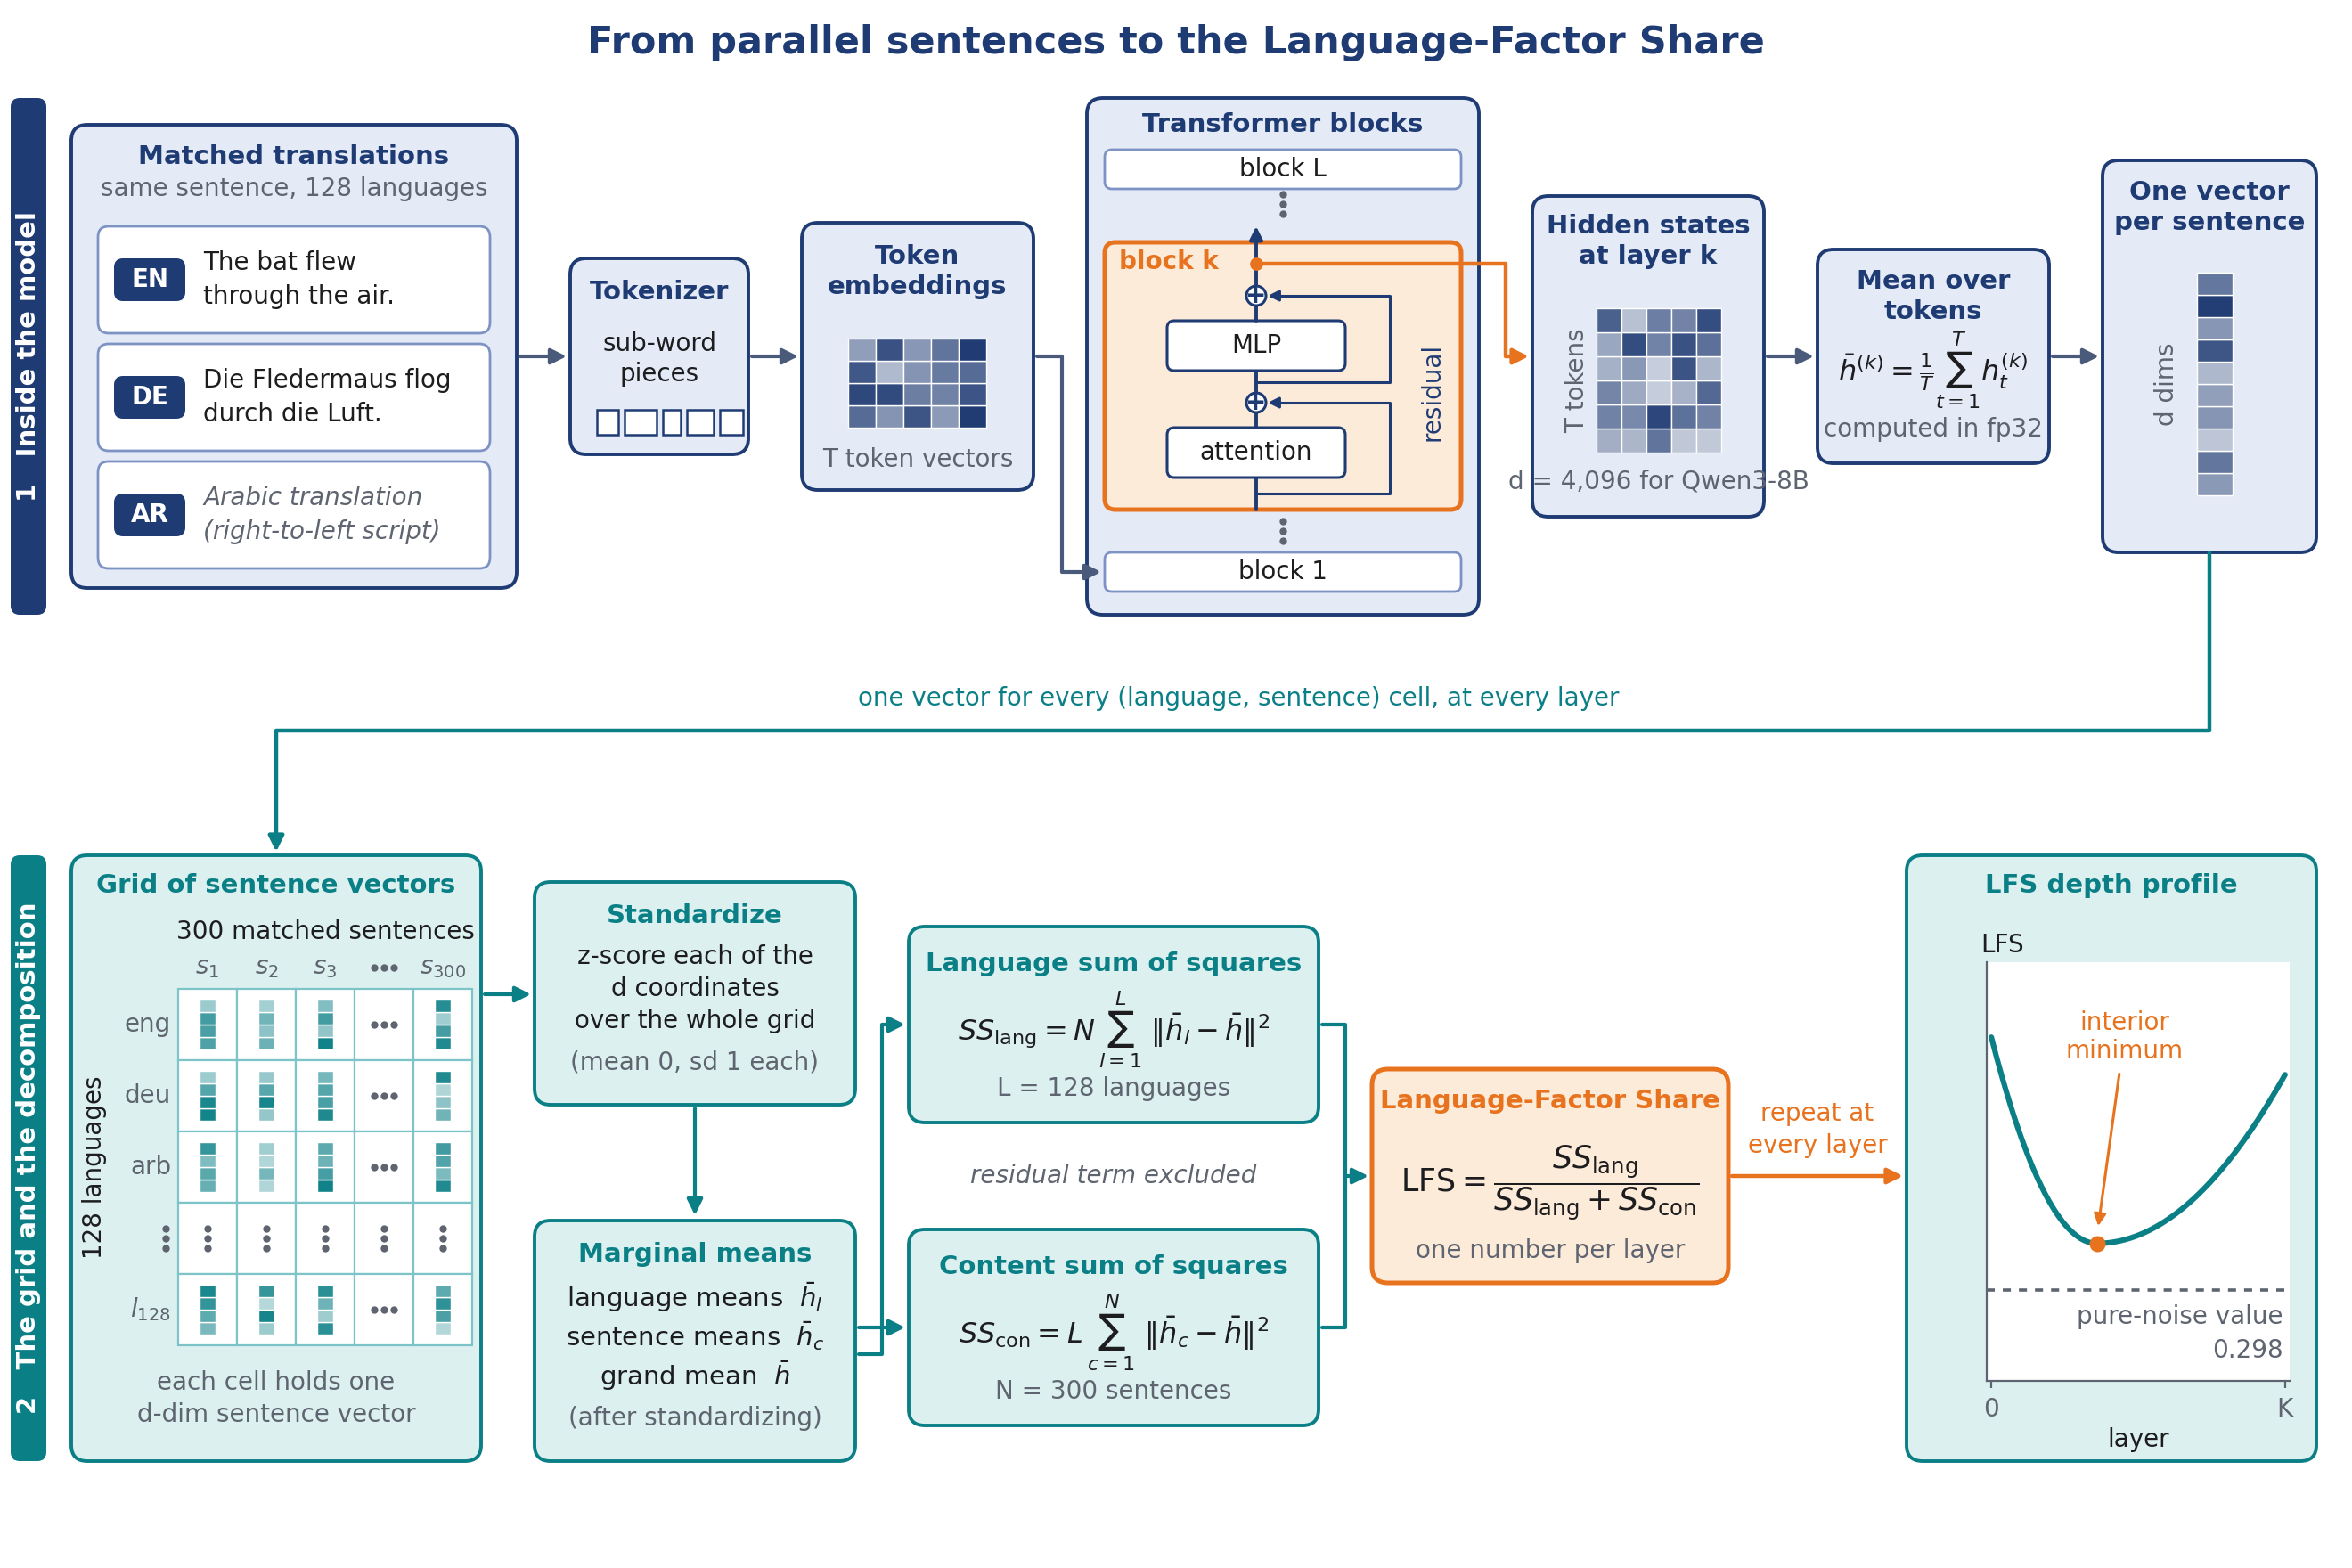
\includegraphics[width=\linewidth]{figs/report/fig22_pipeline_diagram.png}
\caption{The whole measurement on one page: inside the model (top) and the grid with its decomposition (bottom).}\label{fig:pipeline-guide}\end{figure}

\subsection{The table is a three-dimensional array}

Nothing is ever typed into a table. After the forward pass, mean pooling over
tokens gives one vector per (language, sentence) pair. Stacked, they form an
array
\[
X[\ell, c, d], \qquad \ell = 1..128 \text{ languages},\; c = 1..300 \text{ sentences},\; d = 1..4096 \text{ coordinates},
\]
one such array per layer. The example in Chapter~\ref{ch:lfs} is this array
with $L=2$, $N=3$, $D=1$. Everything below is the same array with the real
sizes. Stored on the cluster as \texttt{layer000.npz}, \texttt{layer019.npz},
and so on; the first 300 of the 1,500 stored sentences are the main grid.

\subsection{Raw values at the dip layer}

Table~\ref{tab:rawvals} shows the first five of the 4,096 coordinates for
three sentences in seven languages at layer 19, the dip layer of Qwen3-8B.
These are the numbers the model produced, mean-pooled, before any
standardization. Two things to notice. They are ordinary floating-point
numbers, mostly between $-1$ and $1$. And a language does not announce
itself: nothing in the Arabic rows looks obviously different from the English
rows on these five coordinates. The language effect is spread thinly over
thousands of coordinates and only becomes visible when you average.

\begin{table}[h]\centering\small
\caption{Qwen3-8B-Base, layer 19, mean-pooled hidden states, coordinates 0 to 4.}
\label{tab:rawvals}
\begin{tabular}{llrrrrr}
\toprule
Language & Sentence & $d_0$ & $d_1$ & $d_2$ & $d_3$ & $d_4$ \\
\midrule
eng & 0 & 0.159 & 0.191 & $-0.902$ & 0.012 & 0.651 \\
eng & 1 & $-0.085$ & $-0.811$ & $-0.418$ & $-0.140$ & 0.448 \\
eng & 2 & $-0.928$ & 0.185 & $-0.486$ & $-0.369$ & 0.076 \\
deu & 0 & $-0.236$ & 0.287 & $-0.567$ & $-0.213$ & 0.385 \\
deu & 1 & $-0.453$ & $-0.218$ & $-0.384$ & 0.205 & 0.245 \\
deu & 2 & $-0.439$ & $-0.165$ & $-0.909$ & $-0.071$ & 0.292 \\
fra & 0 & $-0.311$ & $-0.036$ & $-1.171$ & $-0.149$ & 0.051 \\
fra & 1 & $-0.667$ & $-0.311$ & $-0.713$ & $-0.038$ & $-0.171$ \\
fra & 2 & $-0.325$ & $-0.646$ & $-1.328$ & $-0.203$ & $-0.028$ \\
spa & 0 & 0.185 & $-0.504$ & $-0.142$ & 0.032 & 0.064 \\
spa & 1 & $-0.060$ & $-0.774$ & $-0.538$ & 0.124 & 0.112 \\
spa & 2 & $-0.662$ & $-0.279$ & $-1.328$ & 0.145 & $-0.014$ \\
rus & 0 & $-0.207$ & $-0.119$ & $-0.102$ & $-0.014$ & 0.190 \\
rus & 1 & $-0.406$ & $-0.288$ & $-0.161$ & 0.134 & 0.202 \\
rus & 2 & $-0.472$ & $-0.686$ & $-0.541$ & $-0.232$ & 0.210 \\
arb & 0 & $-0.308$ & 0.533 & $-0.108$ & 0.359 & $-0.130$ \\
arb & 1 & $-0.255$ & $-0.182$ & $-0.117$ & 0.415 & 0.001 \\
arb & 2 & $-0.026$ & $-0.048$ & $-0.706$ & 0.257 & $-0.164$ \\
fas & 0 & 0.067 & 0.434 & $-0.257$ & 0.434 & 0.382 \\
fas & 1 & $-0.469$ & 0.403 & $-0.400$ & 0.860 & 0.151 \\
fas & 2 & $-0.259$ & 0.778 & $-0.703$ & 0.540 & $-0.094$ \\
\bottomrule
\end{tabular}
\end{table}

\subsection{The table on one coordinate, with real means}

Fix one coordinate and the array becomes exactly the Chapter~\ref{ch:lfs}
table, 128 rows by 300 columns. Table~\ref{tab:onecoord} shows coordinate
1082 at layer 19, a coordinate of typical spread, for the seven languages and
three sentences, together with the three kinds of mean:

\begin{itemize}[leftmargin=1.6cm]
\item[language mean] the mean of that language's row over all 300 sentences
(the ``column mean'' of the small example, where languages were columns);
\item[sentence mean] the mean of that sentence's column over all 128
languages;
\item[grand mean] the mean of all $128 \times 300 = 38{,}400$ cells.
\end{itemize}

\begin{table}[h]\centering\small
\caption{Coordinate 1082, layer 19. Values for three sentences, then each language's mean over all 300 sentences. The sentence means are over all 128 languages.}
\label{tab:onecoord}
\begin{tabular}{lrrrr}
\toprule
Language & sentence 0 & sentence 1 & sentence 2 & language mean (300 sentences) \\
\midrule
eng & 0.209 & 0.315 & 0.759 & 0.155 \\
deu & 0.369 & 0.413 & 0.841 & 0.207 \\
fra & 0.406 & 0.483 & 0.587 & 0.220 \\
spa & 0.142 & 0.186 & 0.657 & 0.240 \\
rus & 0.554 & 0.120 & 0.346 & 0.121 \\
arb & 0.210 & 0.453 & 0.401 & 0.321 \\
fas & 0.445 & 0.528 & 0.606 & 0.274 \\
\midrule
sentence mean (128 languages) & 0.148 & 0.244 & 0.323 & grand mean 0.181 \\
\bottomrule
\end{tabular}
\end{table}

On this single coordinate the language sum of squares is
$300 \sum_\ell (\bar x_\ell - \bar x)^2 = 637.9$ and the sentence sum of
squares is $128 \sum_c (\bar x_c - \bar x)^2 = 634.5$, so the language share
of this coordinate is $0.501$. That is one coordinate's vote.

\subsection{``Coordinate by coordinate'' means 4,096 such tables}

LFS does not pick one coordinate. It computes the two sums of squares on
every coordinate and adds them up. In vector form that is what
$\|\bar{\mathbf z}_\ell - \bar{\mathbf z}\|^2$ does: a squared norm is a sum
over coordinates of squared differences, so the language sum of squares of
the whole grid is the sum of the 4,096 per-coordinate language sums of
squares. The code never builds 4,096 tables; it takes means along the axes of
the array (\texttt{X.mean(1)} for language means, \texttt{X.mean(0)} for
sentence means, \texttt{X.mean((0,1))} for the grand mean) and sums the
squared differences over the coordinate axis.

\subsection{Why standardizing first is not optional}

Here is what the raw array looks like at layer 19 before standardization.
The median coordinate has a standard deviation of $0.26$ across the 38,400
cells. Coordinate 2276 has a mean of $224$ and a standard deviation of
$162$. It is a massive activation, a single coordinate the model uses as an
internal bias that is hundreds of times larger than everything else. Its
values for the same seven languages are in Table~\ref{tab:massive}.

\begin{table}[h]\centering\small
\caption{Coordinate 2276, layer 19, the largest-spread coordinate. Same layout as Table~\ref{tab:onecoord}.}
\label{tab:massive}
\begin{tabular}{lrrrr}
\toprule
Language & sentence 0 & sentence 1 & sentence 2 & language mean \\
\midrule
eng & 718.0 & 315.8 & 450.3 & 454.9 \\
deu & 407.0 & 203.8 & 263.5 & 298.8 \\
fra & 308.8 & 221.8 & 337.5 & 299.1 \\
spa & 237.8 & 208.5 & 398.3 & 309.4 \\
rus & 339.3 & 134.4 & 285.3 & 249.5 \\
arb & 287.3 & 215.1 & 355.5 & 288.8 \\
fas & 265.3 & 200.0 & 235.9 & 200.8 \\
\midrule
sentence mean & 304.0 & 174.3 & 249.0 & grand mean 224.4 \\
\bottomrule
\end{tabular}
\end{table}

Because sums of squares grow with the square of the scale, this one
coordinate carries $92.8$ percent of the total sum of squares of the whole
layer; the top ten coordinates carry $96.5$ percent; the other 4,086
coordinates share the remaining few percent. If LFS were computed on the raw
array, the language sum of squares would be $89.7$ percent coordinate 2276
and the sentence sum of squares $94.9$ percent coordinate 2276, and the
result, $0.347$, would be the language share of one neuron (on its own that
coordinate's share is $0.334$). The other 4,095 coordinates would be
outvoted. That is what ``a single huge dimension dominates'' means: the
metric silently becomes a measurement of whatever that coordinate does,
which here is mostly a bias term with some content in it.

Standardization divides each coordinate by its own standard deviation across
the grid. After that, coordinate 2276 carries $0.02$ percent of the language
sum of squares and $0.06$ percent of the sentence sum of squares, in line
with the $0.024$ percent a coordinate would carry if all were equal, and the
layer-19 LFS is $0.608$. The standardized values are unit-scale numbers: the
English sentence 0 becomes $[1.32, 0.08, -2.41, -0.39, 2.07]$ on the first
five coordinates.

At layer 0 the same check shows why the effect is layer-dependent. There, the
largest coordinate carries $0.8$ percent of the total, the raw and
standardized LFS are $0.929$ and $0.945$, and the mean vector norm is $0.5$.
By layer 19 the mean norm is $240$, a five-hundred-fold growth through the
network, almost all of it in a handful of coordinates. This is the same fact
behind the collapse blind spot in the paper: the raw scale of a
representation is information, and a ratio throws it away, so the components
and the norm are reported beside the ratio.

\begin{exercise}{watch one coordinate take over}
\begin{lstlisting}
import numpy as np
rng = np.random.default_rng(0)
L, N, D = 8, 50, 64
lang = rng.normal(0, 1.0, (L, 1, D)); sent = rng.normal(0, 1.5, (1, N, D))
X = lang + sent + rng.normal(0, 0.5, (L, N, D))    # additive grid, language weaker than content
def lfs(X):
    mu = X.mean((0, 1)); ml = X.mean(1); mc = X.mean(0)
    ssl = X.shape[1] * ((ml - mu)**2).sum(); ssc = X.shape[0] * ((mc - mu)**2).sum()
    return ssl / (ssl + ssc)
def z(X):
    f = X.reshape(-1, X.shape[-1]); return (X - f.mean(0)) / (f.std(0) + 1e-9)
print(round(lfs(X), 3), round(lfs(z(X)), 3))          # similar: no dominant coordinate yet
X[..., 7] += 200 + 160 * rng.normal(size=(L, N))      # one massive coordinate: a per-cell bias, no language structure
print(round(lfs(X), 3), round(lfs(z(X)), 3))          # raw LFS collapses toward that coordinate's own share; standardized LFS barely moves
\end{lstlisting}
Then compute the fraction of the total sum of squares that coordinate 7
carries before and after \texttt{z}. You have reproduced the layer-19
situation of Table~\ref{tab:massive}.
\end{exercise}

\subsection{So, is a table always built?}

Yes, in the only sense that matters: every LFS number in the paper and the
report comes from an array of exactly this shape, languages by sentences by
coordinates, at one layer, standardized coordinate by coordinate, decomposed
into a language part, a sentence part, and a remainder. The grids differ in
size (128 by 300 for the main profiles, 128 by 1,500 for the study
dumps, 116 by 300 for FLORES-200) and in the model, layer, and pooling, but
never in shape or in the arithmetic.
